%!TEX root = ../thesis.tex

\chapter{资料及模式介绍}

\section{原位观测}

\subsection{臭氧探空}

针对强对流天气,本小组成员于2019年7月25日和2020年9月1日,在南京国家基准气候站(31.93$^{\circ}$N,118.90$^{\circ}$E)共释放了五台臭氧探空仪。
为了研究对流的影响,我们分别在对流发生前和对流发生中/对流发生后各释放一次探空。
深对流概况及臭氧探空仪轨迹见图\ref{figure:ozonesonde}(a)和(b)。

具体而言,2019年7月25日发生的对流为热对流,释放的三个臭氧探空均产自中国大气物理研究所(IAP)。
IAP 臭氧探空仪使用电化学浓差电池 (ECC),其完整参数和性能见\citet{Zhang.2014}。
总体而言,从地表到2.5 km平均偏差小于0.3 mPa,9 km以下接近零,9--18 km之间小于0.5 mPa。
释放的第一台IAP臭氧探空仪于7月23日(晴天)05:35 UTC释放,另外两台分别于7月25日05:10 UTC(对流前)和06:35 UTC(对流后)释放。
由于防水故障,对流前释放的探空仪在释放后几秒钟就失去了信号,故而我们选择了7月23日释放的臭氧探空仪作为对流前的数据。
虽然时间间隔为2天,但10 km以上预报的O$_3$剖面最大相对差异通常小于25\%(图\ref{figure:waccm_forcast_o3})。
因此,臭氧日变化不足以解释探空观测到的超过65\%的差异。

此外,两台维萨拉(VAISALA)ECC臭氧探空仪分别于8月31日23:45 UTC(对流前)和9月1日06:10 UTC(对流期间)成功释放。
准备工作及具体操作均遵循标准手册,确保精度优于5\%,且在30 km 以下的精度在$\pm$ (5--10) \% 以内\citep{Smit.2007}。
该次探空试验所捕获的飑线是由冷空气和台风梅萨克(Maysak)外围环流的汇合发展而来的。
值得强调的是,对流期间的臭氧探空仪直接穿入云层,为探索受对流云影响的臭氧提供了独特的机会。


\begin{figure}[htbp]
\centering
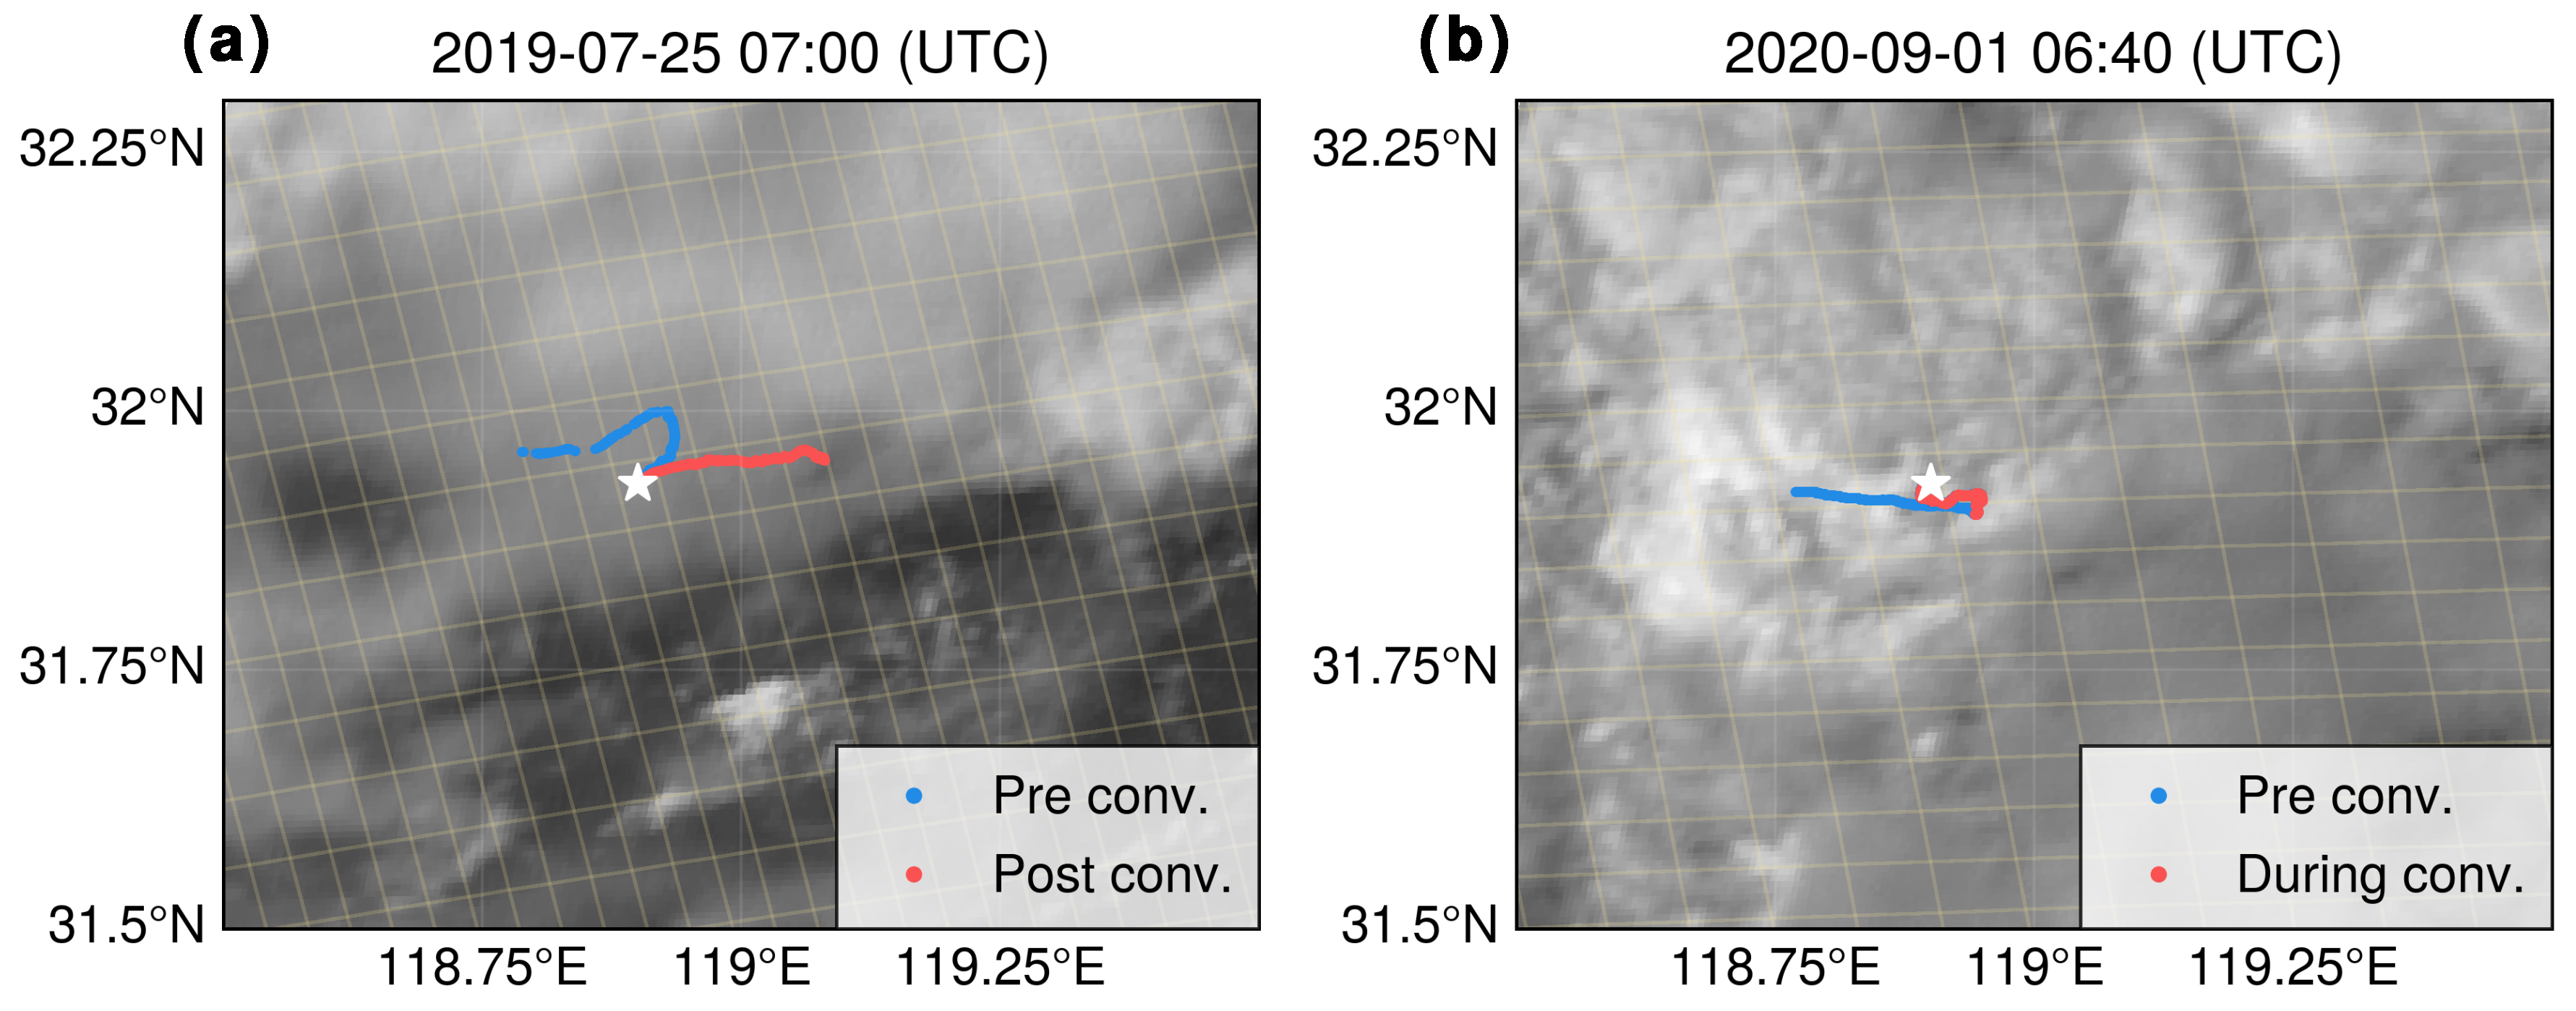
\includegraphics[width=35em]{./figures/ozonesonde.png}
\caption{(a, b) 在对流后/对流中的臭氧探空仪达到约 10 km时,风云4A先进地球静止辐射成像仪(AGRI)可见通道(0.65 $\mu$m)探测到的对流。
对流前的臭氧探空仪轨迹为为蓝色,其他为红色。白星符号代表观测站,细黄线是TROPOMI像素条带。
图(c)和(d)是在对流前(虚线)和对流后/对流期间(实线)探空观测到的O$_3$(红色)和Q$_v$(黑色)廓线。
模式初始(虚线)和对流后或对流期间(实线)的O$_3$廓线为蓝色。
深灰色阴影是50\%的置信区间,浅色是90\%的置信区间,灰线是第一对流层顶。}
\label{figure:ozonesonde}
\end{figure}

\begin{figure}[htbp]
\centering
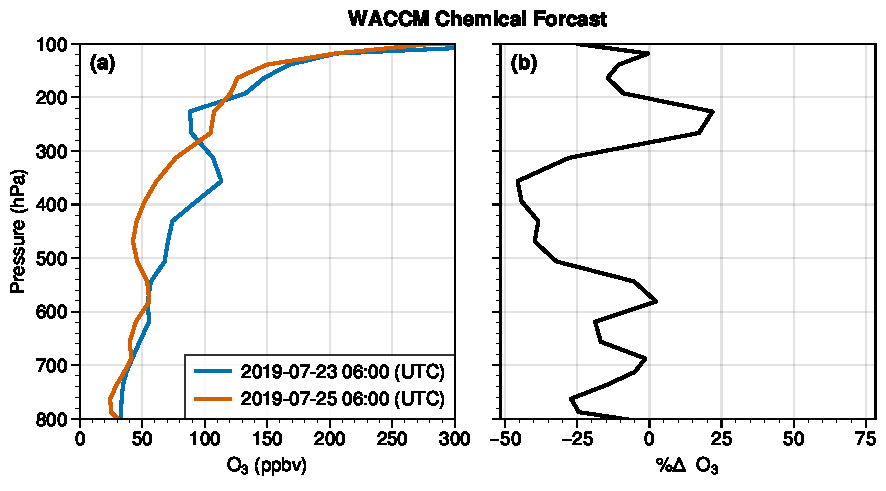
\includegraphics[width=35em]{./figures/waccm_forcast_o3.pdf}
\caption{(a)WACCM预测的区域平均(118.5$^{\circ}$E -- 119.5$^{\circ}$E, 31.5$^{\circ}$N – 32.5$^{\circ}$N)臭氧廓线。
蓝色为对流前,橙色为对流后。(b)为(a)中O$_3$剖面的百分比差异。}
\label{figure:waccm_forcast_o3}
\end{figure}

\subsection{闪电数据集}

\section{卫星观测}

\subsection{臭氧监测仪}
\subsection{对流层观测仪}
\subsection{闪电氮氧化物反演}

\section{模式设置}

\subsection{气象设置}
\subsection{化学设置}
\subsection{闪电资料同化}

